\section{\iso Problem and Related Work}
\label{sec:tqc_problem}

\begin{figure}[ht]
    \centering
    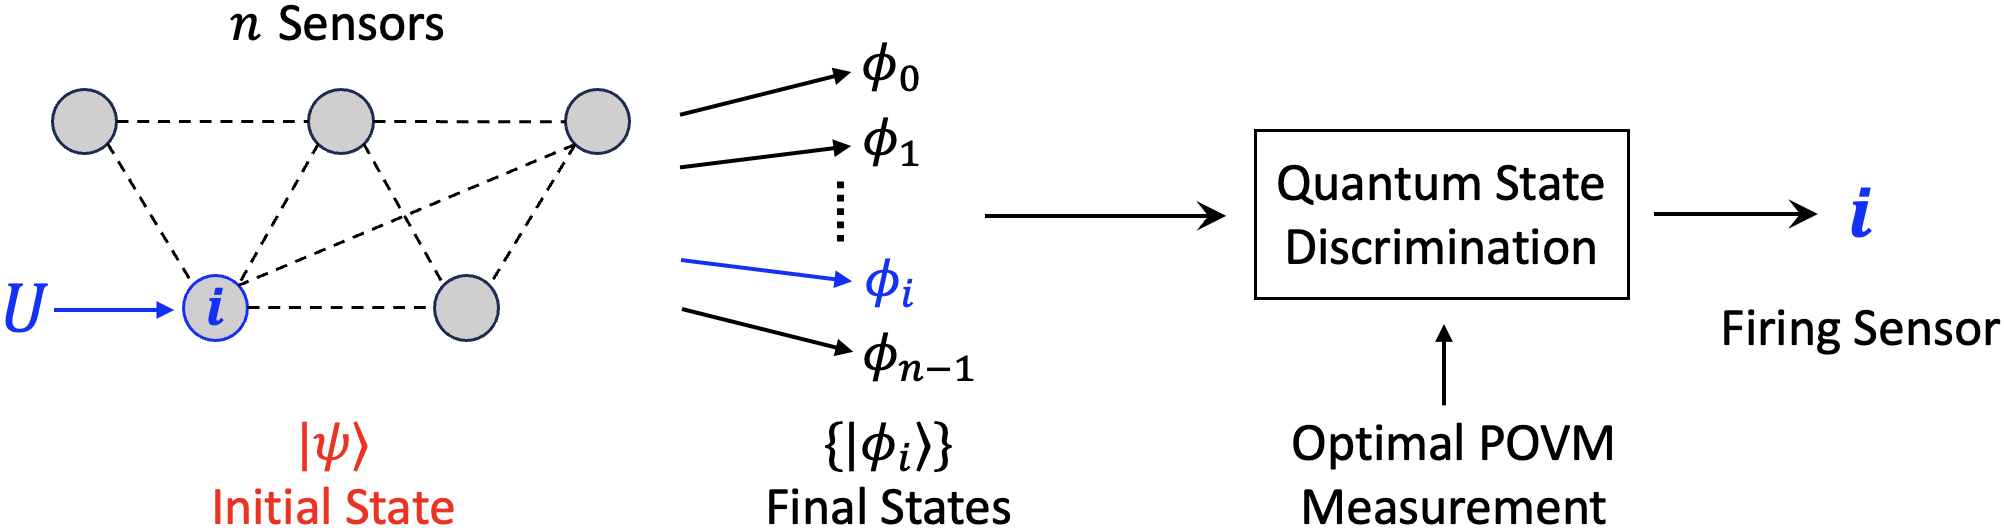
\includegraphics[width=0.9\textwidth]{chapters/tqc/figures/ISO.png}
    \caption{\iso Problem. Given $n$ deployed quantum sensors, an event changes the state of one of the sensors  ($i^{th}$ sensor in the figure) by a unitary operator $U$. Quantum state discrimination with the optimal measurement is used to determine the firing sensor. The \iso problem is to determine the initial state (possibly, entangled) that minimizes the probability of error in discriminating the potential final states. The dashed lines connecting the sensors signify a potential entangled global state.
    } 
    \label{fig:qsn}
\end{figure}

\para{Setting.} Consider $n$ quantum sensors deployed across a geographical area, forming a quantum sensor network. See Fig.~\ref{fig:qsn}. 
Each sensor stores a qubit whose state may potentially change due to an event in the environment.
Let $\ket{\psi}$ denote the initial (possibly entangled) state of the $n$ sensors.
Let $U$ be a unitary operator that represents the impact of an event over a qubit in a sensor;
here, $U$ may describe the rotation of a spin caused by a magnetic field or a phase shift induced in a state of light by a transparent object.
Let the two eigenvectors of $U$ be $\{u_+, u_-\}$, and without loss of generality,
let the corresponding eigenvalues be $\{e^{+i\theta}, e^{-i\theta}\}$
where $\theta \in (0, 180)$ degrees;
thus, $U\ket{u_{\pm}}=e^{\pm i\theta}\ket{u_{\pm}}$.
Let $\ket{\phi_i} = (I^{\otimes i} \otimes U \otimes I^{\otimes (n-i-1)})\ket{\psi}$, 
where $U$ appears in the $i^{th}$ 
position and $i\in \{0, \cdots, n-1 \}$, 
represents the system's state after the event affects the $i^{th}$ sensor. 
{\em We assume that events in our setting affect exactly one sensor with uniform probability.}\footnote{In essence, we assume that sensors are sparsely deployed such that
an event affects at most one sensor, and that the event itself is uniformly likely to occur at the sensor locations. 
If there is no prior information about the event's location, then assuming uniform probability is reasonable.
See \S\ref{sec:extend}, where we consider the generalization of non-uniform probabilities.}
We refer to the $n$ possible resulting states $\{\ket{\phi_i}\}$ as the {\bf final states}; these
final states have an equal prior probability of occurrence on an event.

\softpara{Objective Function $P(\ket{\psi}, U)$.}
When an event results in the system going to a particular final state $\ket{\phi_i}$, 
we want to determine the sensor (i.e., the index $i$) that is impacted by the event by performing a global measurement of the system. For a given setting (i.e.,  $\ket{\psi}$ and $U$), let 
$M(\ket{\psi}, U)$ be the optimal 
{\em positive operator-valued measure} (POVM) measurement for discriminating the
final states $\{\ket{\phi_i}\}$, i.e., 
the measurement that incurs the
minimum probability of error in 
discriminating the
final states $\{\ket{\phi_i}\}$ and thus
determining the index 
$i$ given an unknown final state.
Let $P(\ket{\psi}, U)$ be the (minimum) probability of error incurred by $M(\ket{\psi}, U)$ in discriminating the final states $\{\ket{\phi_i}\}$.

\para{\iso Problem Formulation.} 
Given a number of sensors $n$ and a 
unitary operator $U$, 
the \iso problem to determine the 
initial state $\ket{\psi}$ that minimizes
$P(\ket{\psi}, U)$.
In other words, we wish to determine the initial state $\ket{\psi}$ 
that yields the lowest probability of error in discriminating the final states when
an optimal POVM is used for discrimination.

{\em For clarity of presentation, we consider only the minimum error measurement 
scheme, till the last Section~\ref{subsec:ud} where we extend our results to the unambiguous discrimination measurement scheme.}

\softpara{Potential Applications.}
One of the main applications of detector sensor networks is event localization. 
Assume we have some critical locations to monitor, and we place one quantum detector at each critical location.
Then, a network of quantum detectors, wherein a detector's
state changes (as represented by the unitary $U$), can be used to localize the event occurrence---as the location of the firing detector also gives the event's location. 
The event in the above scenario could be anything that can be represented by a unitary $U$, e.g., 
an event may represent the presence of a magnetic field, an acoustic event (e.g., an explosion), a signal transmission that can be detected, or movement of a detectable object.



\para{Paper Organization.}
The rest of the paper is organized as follows. We end this section with a discussion on related work.
In the following section (\S\ref{sec:three-ortho}), 
we establish a necessary and sufficient condition for \emph{three} final states to be orthogonal---and hence, the existence of an initial state such that 
$P(\ket{\psi}, U) = 0$. 
We generalize the result to an \emph{arbitrary} number of sensors in \S\ref{sec:n-ortho},
and give an optimal solution for the \iso problem when the orthogonality condition is satisfied.
In \S\ref{sec:optimal}, we use the insights from \S\ref{sec:n-ortho} to derive a conjectured optimal solution for an arbitrary $U$ and the number of sensors; in the section, we also provide a pathway to proving the conjecture. 
In the following sections, we develop search-based heuristics for the problem (\S\ref{sec:searching}) and use these heuristics to 
empirically validate our conjectured solution through simulations (\S\ref{sec:sim}).
In \S\ref{sec:extend}, we consider generalizations related to 
unambiguous discrimination measurement, non-uniform prior probabilities, and quantum noise.
Finally in \S\ref{sec:tqc-conclusion}, we conclude and discuss some potential future work.

\subsection{Related Work}
\label{sec:related}

\para{Continuous Parameter Estimation using Quantum Sensors.}
In prior works~\cite{Eldredge_2018,Rubio_2020}, protocols have been studied for estimation of a single parameter using multiple sensors~\cite{Giovannetti_2011}, multiple parameters~\cite{mpe_2018,mpe_2020}, a single linear function over parameters~\cite{Eldredge_2018,mpe_2018,Sidhu_2020}, and multiple linear functions~\cite{Rubio_2020,Altenburg_2019}. 
Quantum state estimation considering nuisance parameters is reviewed in~\cite{Suzuki_2020}.
These and many other works~\cite{Eldredge_2018,mpe_2018,Jacobs_2018} have also
investigated whether the entanglement of sensors offers any advantage 
in improving the estimation accuracy. Some of the above works have optimized
the measurement protocols (e.g, ~\cite{Eldredge_2018,PhysRevA.qsn}) in the addressed
settings, but none of the above works have addressed the problem of initial state optimization.
To the best of our knowledge, all prior works have modeled the 
sensed parameters in the continuous domain, e.g., these parameters could be the 
strength of a magnetic field at different locations. In contrast, in some sense, our work focuses on the estimation of discrete-valued parameters. 

% To the best of our knowledge, all prior (including the above) works have modeled the 
% sensed parameters in the continuous domain; e.g., these parameters could be the 
% strength of a magnetic field at different locations. 
% In contrast, in some sense, our work is focuses on estimation of discrete-valued parameters. 
% Estimating discrete values should be fundamentally a simpler problem than estimating
% their continuous value---as we are seeking much less information. \red{Neither of these
% works have considered optimization of initial state; optimization of measurements yet.}

\para{Optimal State Discrimination.}
There has been a lot of work on quantum state discrimination~\cite{bergou-review-2007,bergou2004,Bae_2015,Barnett-review} -- wherein the goal is to determine the 
optimal measurement protocol to minimize the probability of error
in discriminating a set of given states. 
A closed-form expression is known only for two states and very specialized cases for a larger
number of states. However, numerical techniques exist (e.g., SDP-based~\cite {semidefinite}).
%%%%%%
Our work differs in the following ways: (i) The set of final states we want to discriminate is very 
specialized. (ii) Our goal is to optimize the initial state---that minimizes the probability of error using an optimal POVM (in some sense, we implicitly assume that an optimal POVM for a given set of final states can be derived). 


% Recently, Zhuang and Zhang~\cite{slaen} developed a classical supervised learning
% architecture called SLAEN (supervised learning assisted by an entangled network) wherein they use variational optical 
% circuits to learn and create an optimized entangled probe/initial state and measurement setting, for supervised learning tasks. 
% \magenta{~\cite{Koczor_2020} similarly optimizes the initial state using a variation circuit, but they also consider noise.}

%%%%%%%%%%%%%



\para{Initial State Optimization.} 
Recent works have used variational circuits to seek an optimized probe 
state for a set of sensors, in the context of classical supervised learning~\cite{slaen}
and (continuous) parameter estimation~\cite{Koczor_2020} under noise. 
\eat{\cite{ouyang22-symmetric} shows that symmetric probe states are good candidates for robust quantum metrology.}
%%%%%%%%%%%%%%%%%%%
In additional, a recent work~\cite{ehrenberg} investigates estimation accuracy
with different levels of entanglements 
for measuring a linear combination of field amplitudes.
In contrast, we seek provably optimal initial state solutions. 
To the best of our knowledge, the only other work that has 
investigated the initial state optimization problem is 
our recent preliminary work~\cite{Hillery_2023} where we address the same 
problem as in this paper. 
In~\cite{Hillery_2023}, we give an optimal solution for the case of $n=2$ sensors,
and, for the general case of  $n$ sensor, we derive 
close-form expressions for the probability of error 
for a heuristic solution for a restricted class of initial 
states, and investigate the benefit of entanglement in the
initial state. 
%%%%%%%%%%%%%%%%%%%%
% In this paper, 
% we derive conditions for orthogonality, provide a conjecture optimal solution 
% that we believe to be very likely true, and corroborate the conjecture through
% extensive simulations using multiple search heuristics that seem
% to deliver near-optimal solution.

% \blue{This paper is closely related to our other paper~\cite{mark-22} and the two papers have the same background. The main differences are as follows.
% \begin{enumerate}
%     \item Problem formulation. 
%     In~\cite{mark-22}, choosing the initial state of the sensors and choosing the measurement are both considered. 
%     In this paper, however, we mainly focus on choosing the initial state. 
%     Choosing the measurement becomes more trivial as we resort to a numerical solver (SDP) instead of an analytical method used in~\cite{mark-22} and assume the numerical solver will always give us an optimal measurement.
%     \item The range of $\theta$. In~\cite{mark-22}, the range of $\theta$ is only $[0, \pi/4]$ (the paper says $[-\pi/4, \pi/4]$, but negative degrees are symmetric to positive degrees, thus ignored).
%     In this paper, we consider a broader range of $\theta$, $[0, \pi]$, and give the Theorem~\ref{thm:nsensors} that provides the condition of $\theta$ when the perfect discrimination of the final states exists in our problem, i.e., the orthogonality of the final states.
%     \item Assumption. In the range of $[0, \pi/4]$, which~\cite{mark-22} considers, the final states will never be mutually orthogonal, and the paper \emph{suggests} an optimal initial state under the assumption of the initial state being symmetric.
%     In this paper, we \emph{conjecture} an optimal initial state under a range of $\theta$ when the final states being mutually orthogonal is impossible (by Theorem~\ref{thm:nsensors}), and the conjectured optimal initial state happens to be symmetric.
%     \item Minor.~\cite{mark-22} considered the case of no-detection fired, while this paper didn't consider it. 
%     ~\cite{mark-22} considered unambiguous discrimination while this paper also didn't.
%     \item Objective is different.
% \end{enumerate}
% }


